\documentclass{article}
\usepackage{lmodern}
\renewcommand{\rmdefault}{lmss}
\usepackage[T1]{fontenc}
\usepackage[utf8]{inputenc}
\usepackage{float}
\usepackage{graphicx}
\usepackage[margin=1in]{geometry}
\usepackage{titlesec}
\usepackage{inconsolata}
\usepackage{hyperref}
\usepackage{subcaption}
\usepackage{amsmath}
\usepackage{amssymb}
\usepackage{mathtools}
\usepackage{indentfirst}
\newcommand{\code}[1]{{\fontfamily{zi4} \selectfont{#1}}}
\newcommand{\sectionbreak}{\clearpage}
\setcounter{secnumdepth}{2}
\usepackage{fancyhdr}
\pagestyle{fancy}
\fancyhf{}
\fancyhead[L]{\leftmark}
\fancyhead[R]{\thepage}
\renewcommand{\headrulewidth}{0.4pt}
\DeclarePairedDelimiter\floor{\lfloor}{\rfloor}
\hypersetup{colorlinks=true, urlcolor=cyan, linkcolor=[rgb]{0.05,0.05,0.05}}

\begin{document}

\begin{titlepage}
   \begin{center}
       \vspace*{1cm}

       \huge{\textbf{Deep Learning}}
          
       \vspace{0.5cm}

       \Large{Shanmugha Balan S V}
      
   \end{center}
\end{titlepage}

\tableofcontents

\section*{Preface}
This is my notes for Deep Learning which I've prepared from a variety of sources. Most of the basics, optimization, convolutional networks and recurrent networks are from the \href{https://www.coursera.org/specializations/deep-learning}{Deep Learning Specialization} by Andrew Ng on Coursera. Most of the code for this is in \href{https://github.com/sbalan7/LearningDeepLearning}{my repository} and it contains all the assignments from this course. Convolutional Networks also features a small amount of content from CS231n: Convolutional Neural Networks for Visual Recognition, a course by Stanford Online. 

Far from complete, this pdf could use much more information than it currently holds. If you want to contribute something to this pdf, or if you find any errors in this, please open a pull request for this \href{https://github.com/sbalan7/LearningDeepLearning/}{repository}.

Version 8.4 
January 2021

\section{Neural Network Basics}

\subsection{Forward Propagation}

The perceptron is the building block of a neural network. It can be considered as a node through which an input to the network flows. The inputs are multiplied by weights which are summed and are passed through an activation function which enforces non-linearity to give an output. The weights are in the form of a matrix, which is of the form $n^{[l]} \times n^{[l-1]}$, where $n^{[k]}$ is the number of units in the $k^{th}$ layer. Sometimes, these are passed through a bias term (of shape $n^{[l]} \times 1$, and then through the activation function to give the output. In other words,
$$\widehat{y} = \sigma(w_0 + X^TW)$$
As a general notation, for the rest of the document the following hold.\\
$m$ Number of examples in the training set\\
$n_x$ Size of the input\\
$n_y$ Size of the output\\
${n_h}^{[l]}$ The hidden units in the $l^{th}$ layer\\
$L$ Layers in the network

\begin{figure}[h]
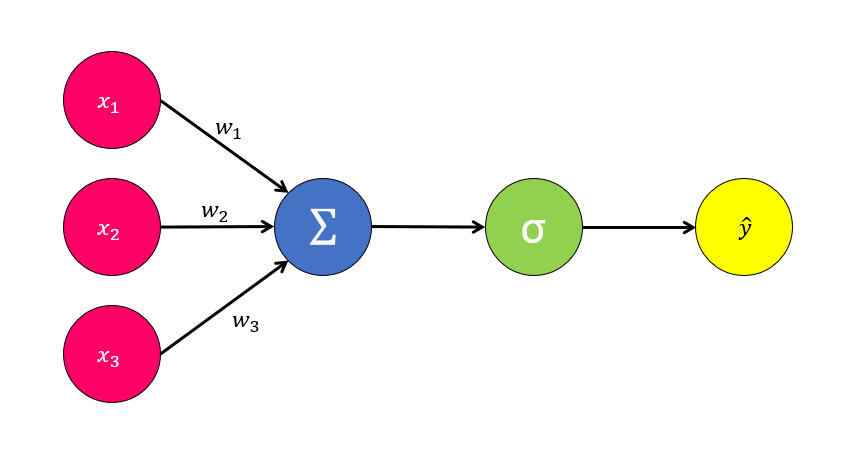
\includegraphics[width=10cm]{Images/perceptron.png}
\centering
\caption{A simple neural network}
\end{figure}

One iteration forward through the neural network is known as forward propagation. To start with forward propagation, every perceptron is initialized to a random value close to zero. This helps in breaking symmetry, and ensuring the nodes in the hidden layers all don't perform the same computation. Now with our random weight matrix, we perform the first step of linear forward propagation, and then we activate it. The final part of forward propagation is looking back and checking the loss. Mathematically, we can describe forward propagation as
$$ For\ a\ layer\ l,\ with\ input\ a^{[l-1]},\ we\ output\ a^{[l]}\ and\ a\ tuple\ with\ W^{[l]}\ and\ b^{[l]} $$
$$ Z^{[l]} = W^{[l]} \cdot a^{[l-1]} + b^{[l]} $$
$$ a^{[l]} = g^{[l]} (z^{[l]}) $$

\subsection{Activation Functions}

Activation functions are used to introduce non-linearities in a neural network. They allow us to compute arbitrarily complex partitions of data, while linear activations provide linear outputs every time. An activation function must be so chosen so that it is inexpensive to calculate, as it would have to be performed for every node. The activation function also mustn't shift the gradient towards zero while performing gradient descent in back propagation. Some common activation functions are 

\textbf{Sigmoid function}, which is almost exclusively used only for binary classification. It produces values in the range of 0 to 1 - it is not zero centred. The softmax is a slight variation of the sigmoid, which again produces values in the range 0 to 1, and is used in multi-class classification problems. The hyperbolic tangent activation function, the $tanh(z)$ is similar to the sigmoid, but it is zero centred.

$$\sigma(z) = \frac{1}{1+e^{-z}}$$

\textbf{ReLU} or the Rectified Linear Unit is the most widely used activation function and is highly optimized for gradient descent. The ReLU is defined as $max(0, x)$. Sometimes, a variant known as leaky ReLU is used, where we consider a hyperparameter $a$ close to 0, generally as 0.01, and redefine leaky ReLU as $max(ax, x)$, which ensures that nodes in 0 don't die out without learning anything.


\subsection{Loss Functions}

Loss functions or cost functions calculate how different the prediction is to the actual value, and evaluates how the model should change its parameters while learning. Over the course of running the model multiple times, we attempt to reduce the value of the cost. The most basic cost function and the most obvious one would be the mean squared error loss function, which is
$$J(a, y) = \frac{1}{m} \sum_{i=1}^{m}(a-y)^2$$
The MSE would work better for regression problems and the kind. For classification, we need a different approach, for which we use cross entropy loss, given by
$$J(a, y) = -\frac{1}{m} \sum_{i=1}^{m}(y loga + (1-y)log(1-a))$$
To minimise this loss, we alter our weights and biases and begin learning from the data by starting back propagation.

\subsection{Back Propagation}

In back propagation, we evaluate how good our prediction is, and try to improve it by changing the parameters on which the prediction is made. To start, we pick a random point from the loss function, compute the gradient there, and move away from the direction of increase of the gradient till we go into a valley. We exploit chain rule here to target every layer in the neural network. The equation of back propagation, for a parameter $\theta$ and a learning rate $\alpha$ is
$$ \theta^{[l]} = \theta^{[l]} - \alpha d \theta^{[l]}$$
The learning rate controls how large of a step the gradient descent algorithm takes towards the bottom. It's value mustn't be too large, as it can bounce back and forth between the two walls in the valley. If it's too small, it will take forever to get down.

Gradient descent is the more calculus heavy part of neural networks. Mathematically, the various parts of gradient descent can be summarised in the following equations. Again we iterate through the $L$ layers of the network, with $l$ as any layer in it.

$$\frac{\partial L}{\partial Z^{[l]}} = da^{[l]} \times (g^{[l]})'(z^{[l]}) \equiv dZ^{[l]}$$
$$\frac{\partial J}{\partial W^{[l]}} = \frac{1}{m} dZ^{[l]} \cdot (A^{[l-1]})^T \equiv dW^{[l]}$$
$$\frac{\partial J}{\partial b^{[l]}} = \frac{1}{m} \sum_{i=1}^{m} dz^{[l]} \equiv db^{[l]}$$
$$\frac{\partial L}{\partial A^{[l-1]}} = (W^{[l]})^T \cdot dz^{[l]} \equiv dA^{[l-1]}$$

Computationally, gradient descent is implemented in these helper functions.

\begin{figure}[H]
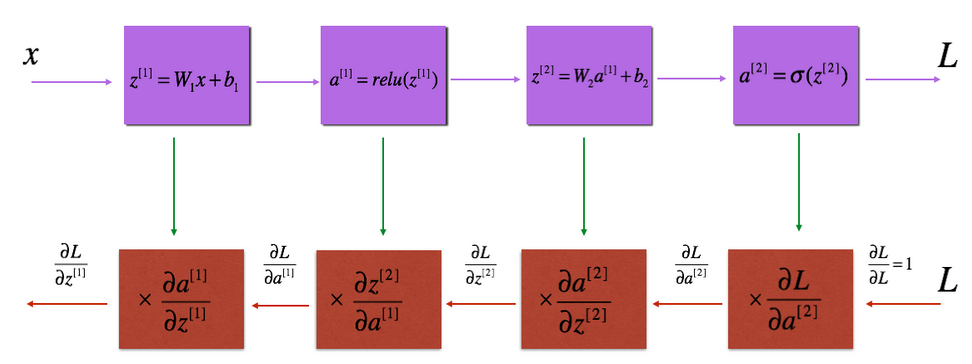
\includegraphics[width=15cm]{Images/twolayernn.png}
\centering
\caption{Forward and Backward Propagation in a two layered neural network}
\end{figure}

\subsection{Oh, yeah. It's all coming together}

Putting together every helper function we have defined before, we make a binary classification model with $L$ layers down here. Since Rome wasn't built in a day, we train our model by running it multiple times over the number of epochs. The learning rate is the parameter which controls how fast we gradient descend. To predict something with the neural network, we simply perform one iteration of forward propagation without the loss, but with a classifier instead, based off the value outputted.


\section{Setting up a Neural Network System}

Applied Machine Learning is a highly iterative process, where you have to individually test out the best possible features for your neural network. You must individually pick out and decide how many layers your network should have, what is the best learning rate, what activation functions to use, and so on. To integrate the process of learning from the data, we must first look to our data at hand. We have to split it into a training set, a development set and a testing set. 

\subsection{Development Set and Test Set}

The development set and test set elements are picked from the complete dataset. Usually the split is in a 60-20-20 ratio for smaller datasets, but for larger ones, only a few thousand examples may be needed for its purpose. These elements must be from the same distribution to get consistent results, from trying to achieve the same target across training, development and testing. The training set can have a slightly different distribution, but it is absolutely essential that the test and development set have the same distribution. The development set would give a good idea of best values of hyperparameters to use. The testing set would provide a platform to test if these values are really good, and would give a final confidence score for the model. The bias in the score which can generally be improved as in the above mentioned section, is the difference between human error and training error. The definition becomes slightly vague as the network surpasses human accuracy, but again, we wouldn't require such a metric at that situation. This bias can be reduced with larger models, the optimization algorithms below or hyperparameter search. The difference between the training error and the development set error gives the variance. This error can be reduced with larger training data or regularization. 

\subsection{Bias and Variance}

When our model doesn't classify the data properly, the model is underfitting the data, by showing high bias. If you make a classifier which is very complex and fits the data perfectly, you might be overfitting to your data, by showing high variance. You can find out if these are the case by comparing the errors in the training set and the development set. If your training error is very low, while the development error is relatively high, your model might be overfitting, or sucking up to the training data - there is a high variance. If however, both your errors are high, then again, your classifier isn't doing well even on the training data - it simply hasn't learned well enough. After preliminary evaluation, if your model has high bias, you can try fixing it by implementing a larger network or by running it through more iterations. Once you have your bias to a permissible level, you evaluate the model on the development set. For reducing variance, you can try adding more data, but when you can't do that, you can try regularization of data.

\subsection{Regularization}

We tried to minimise the cost function $J$ in logistic regression. Here we add some parameters to get
$$J(W, b) = \frac{1}{m} \sum_{i=1}^{m} L(\hat{y^{(i)}}, y^{(i)}) + \frac{\lambda}{2m} ||W||_2^2$$
$$where\ \lambda\ is\ the\ regularization\ parameter\ and$$
$$||W||_2^2 = \sum_{j=1}^{n_x} {w_j}^2 = W^T W$$
This is the $L_2$ regularization, with the $L_2$ norm. If we used $L_1$ norm instead, we would have $L_1$ regularization, but the resulting $W$ vector will have a lot of zeros in it, and becomes "sparse". It doesn't help as much with the learning, so is generally not used. For a neural network, we'd implement the equation as follows.
$$J(W^{[1]}, b^{[1]}, ..., W^{[l]}, b^{[l]}) = \frac{1}{m} \sum_{i=1}^{m} L(\hat{y^{(i)}}, y^{(i)}) + \frac{\lambda}{2m} \sum_{l=1}^L ||W^{[l]}||_F^2$$
Here, we use the Frobenius norm, which is the sum of the square of the elements in the matrix.
$$||W^{[l]}||_F^2 = \sum_{i=1}^{n^{[l]}} \sum_{j=1}^{n^{[l-1]}} ({w_{ij}}^{[l]})^2$$
Now that we have changed our cost function for the network, we must also change the $\frac{\partial J}{\partial w^{[l]}}$ to reflect the new additions. The parameter modification equation, however, stays the same.
$$\frac{\partial J}{\partial w^{[l]}} = \frac{1}{m} dZ^{[l]} \cdot (A^{[l-1]})^T + \frac{\lambda}{m} W^{[l]} \equiv dW^{[l]}$$
$L_2$ regularization is also called weight decay because you are slightly reducing the values of the weights matrix. The values of the weights matrix are penalised for being too large. This forces the model to move away from a complicated classifier to a more linear one, capable of only making simpler decisions. As it moves towards high bias, we find a value which satisfies us enough to make a good classifier. Here is a snippet of pseudocode for implementation of this.

Dropout regularization is another popular technique, where a random number of units in a layer are picked and removed from the network. This creates a smaller, simpler network, which is less likely to over fit to data. Dropout works because any perceptron can't depend on any one perceptron from the previous layer, as it could vanish at random. So it would have to spread out it's weight values into a larger spread so that it doesn't stick to it's training data. A downside to dropout, however is that the cost function isn't as well defined.

Another regularization technique is data augmentation, where we take a random modification of a data point in the dataset and add it to the data set. For example, in an image classification dataset, an image could be flipped, or rotated, or zoomed. Another technique is early stopping. Here, the training error and the development set error and plotted against the number of iterations. From the plot, we can determine the joint minima of the development set error and the training set error, and set our epochs hyperparameter accordingly.

\subsection{Setting up the network}

Normalizing the input data to values from a standard normal distribution also helps in ensuring that we can take larger steps when we perform gradient descent. By setting the mean to zero and standard deviation to 1, the contours of the cost function would become more spherical, and the steps don't have to bounce around between values. One concern would be to use the same mean and standard deviation obtained in the training data while evaluating the test data as well. 

The exploding/vanishing gradients problem occurs with very deep neural networks, where for values beyond slightly larger or slightly below 1, the values of the matrix explode or shrink, respectively. As a result the derivatives also explode or vanish with the weights. This could not mean anything good ever. Just watch out don't dewit. Training will take forever with teeny steps when the gradient is small, and the steps might bounce out when the gradient is big.

Initialising the weights matrix to zeros is useless, as it just outputs zero for every example. The network fails to break symmetry. Initialising the weights matrix to large random values gives an initially high cost, but reduces with epochs. Poor initialization can also lead to vanishing or exploding gradients, so we initialise the matrix with small random values. The random numbers generated between 0 and 1 are scaled by a factor of $\sqrt{\frac{2}{n^{[l-1]}}}$, which is what He initialization recommends for ReLU activation. Similarly Xavier initialization uses $1$ in the numerator for the same scaling factor. 

Numerically, the gradient is better approximated when we approach it from both sides. So, for the derivative at a point $\theta$ for a function $f$,
$$f'(\theta) \approx \frac{f(\theta+\epsilon) - f(\theta-\epsilon)}{2\epsilon}$$

Gradient checking is a procedure by which we can check the implementation of back propagation. To start, we use a concatenate function, to make a giant vector $\theta$ composed of $W^{[l]}$ and $b^{[l]}$ and a giant vector $d\theta$ composed of $dW^{[l]}$ and $db^{[l]}$. $\theta$ and $d\theta$ have the same dimensions as $W^{[l]}$ and $dW^{[l]}$ will have the same dimensions. Gradient checking is only a debugging step, and must not be used in training. The value of $d\theta$ will have to account for regularization, if it is implemented. Gradient checking does not work when you perform dropouts. 

\subsection{Extra Stuff}

Also read - transfer learning, multi-task learning and end-to-end learning.



\section{Optimization of a Neural Network}

\subsection{Orthogonalization}
Orthogonalization is the process by which we make our hyperparameter tuning easier. By orthogonalization, we identify and isolate the ways by which we can tune a hyperparameter instead of letting it be dependent on multiple values. So, we try to have orthogonal variation instead of a linear combination. To do this properly, first we fit the training set well with respect to the cost function. Training a larger network and better optimization algorithms can fix issues here. Then we move on to adjust the development set. Regularization and a larger TRAINING set are possible fixes. Finally, the test set is evaluated on the cost function, and issues can be fixed with a larger DEVELOPMENT set. If despite all this, the model doesn't perform well in the real world, the development set or the cost function will have to be modified. The cost function can be varied to accommodate for any possible biases in data. 

\subsection{Metrics}
Considering we have two different parameters on which we decide the hyperparameter set for training a model. We chose a trade off by calculating one metric from all dependent parameters and choose the hyperparameter set from this one metric. This metric is called single number evaluation metric. We also have two more types of metrics - the satisficing metric and the optimizing metric. We always want to have the best possible values for an optimizing metric. Simultaneously, we try to restrict the optimizing metric with the conditions of the satisficing metric. Hence, the optimizing metric(s) is(are) the best possible value(s) for a given constraint placed on the satisfying metric(s).

\subsection{Mini Batches}

For large datasets, gradient descent takes a long time as the model has to compute the step for the whole dataset over and over again. To counter this, we split our input and output data into smaller mini batches. We split the training data into $X^{\{t\}}$ and testing data into $Y^{\{t\}}$. If we consider batches of size m, they compose of the entire original dataset, and hence we are just performing batch gradient descent. For large training sets, this is computationally expensive and hence takes a lot of time. If we consider batches of size 1, we have m batches where each batch is just one training data pair. This is called stochastic gradient descent. This is not perfect as it doesn't point out to the exact minimum and stay there, rather it hovers around the region where the values are minimum. The ideal values to consider for the size of the mini batch would hence be somewhere in $(1, m)$. 

The main pro going for mini batches is that allows for the vectorization of back propagation. This would result in faster calculation. Ideal mini batch sizes are 64 through 512, in powers of 2. However, for small-ish training sets (m ~ 2000), batch gradient descent isn't too slow. For one pass through the training set, or one epoch, we pass through all the mini batches, performing forward and back propagation on one $X^{\{t\}}$ - $Y^{\{t\}}$ pair.

\subsection{Exponentially Weighted Averages}

An exponentially weighted moving average is a is a response filter which applies exponentially decreasing weights to old data. It is given by the following recursively defined equation.
$$v_t = \beta v_{t-1} + (1-\beta)\theta_t$$
For large $\beta$, we get a smooth curve representing the average of the data points, but there is some latency, as the newer values get bogged down and take a while to manifest. For smaller $\beta$, the curve is very noisy, but it is a fast response curve and bends to newer data. Taking $v_0$ to be 0 causes some problems in the beginning where the average isn't an accurate representation of the data, as the value is pushed down by the initial value. This can be corrected by considering the following equation. 
$$v_{corrected} = \frac{v_t}{1-\beta^t}$$
The $v_{corrected}$ undoes the bias initially for smaller $t$ but becomes negligibly different as $t$ gets larger.

Gradient descent can be sped up with this. While we are performing gradient descent, we want a faster learning rate to power down the slope and find the minimum as fast as possible. However a larger learning rate may result in the step overshooting across the contour. Hence there is a check placed on the upper limit as the steps oscillate back and forth, converging at the minimum. With the weighted average, we can "dampen" these oscillations and help gradient descent take steps which oscillate less, forcing it to accelerate downwards instead. The equation can be modified as follows.
$$v_{d \theta} = \beta v_{d \theta} + (1-\beta)\theta$$
$$\theta = \theta - \alpha v_{d \theta}$$

This gives us two hyperparameters - $\alpha$ and $\beta$. $\alpha$ as we already saw is the learning rate. The hyperparameter $\beta$ is generally set to be $0.9$.

\subsection{RMSprop}

The RMSprop algorithm modifies the gradient descent equations as follows. It first calculates the derivative $d \theta$ normally. 
$$S_{d \theta} = \beta S_{d \theta} + (1-\beta) {d \theta}^2$$
$$\theta = \theta - \alpha \frac{d \theta}{\sqrt{S_{d \theta}}}$$

This algorithm works because we can consider the two possible suspects for $\theta$ - $W$ and $b$ to be components which cause the accelerated descent and the oscillatory divergence. The $S_{dW}$ we compute will be relatively small, while the $S_{db}$ that we compute will be relatively large. Hence, the square root in the denominator of the update equation forces smaller changes to the bias and larger changes to the weights matrix, hence causing a faster descent. To prevent the value of the update term exploding too much, a small constant $\epsilon$ is usually added. This ensures numerical stability of the term. 

\subsection{Adam Optimization Algorithm}

The Adam optimization algorithm combines the effect of mini batches and RMSprop. Mathematically, we represent the algorithm as this.
$$ Initialize\ v_{dW} = 0, S_{dW} = 0, v_{db} = 0, S_{db} = 0$$
$$ On\ every\ iteration\ of\ a\ mini\ batch\ t,\ compute\ dW\ and\ db$$
$$v_{d W} = \beta_1 v_{d W} + (1-\beta_1)W \hspace{1cm} v_{d b} = \beta_1 v_{d b} + (1-\beta_1)b$$
$$S_{d W} = \beta_2 S_{d W} + (1-\beta_2) {d W}^2 \hspace{1cm} S_{d b} = \beta_2 S_{d b} + (1-\beta_2) {d b}^2$$
$$V_{dW}^{corrected} = \frac{V_{dW}}{1-{\beta_1}^t} \hspace{1cm} V_{db}^{corrected} = \frac{V_{db}}{1-{\beta_1}^t}$$
$$S_{dW}^{corrected} = \frac{S_{dW}}{1-{\beta_2}^t} \hspace{1cm} S_{db}^{corrected} = \frac{S_{db}}{1-{\beta_2}^t}$$
$$W = W - \alpha \frac{V_{dW}^{corrected}}{\sqrt{S_{dw}}+\epsilon} \hspace{1cm} b = b - \alpha \frac{V_{db}^{corrected}}{\sqrt{S_{db}}+\epsilon}$$
This algorithm is a versatile and widely used algorithm adaptable to a large variety of neural networks. There are four hyperparameters to be used in this algorithm. $\alpha$ is the learning rate which varies with every model, and will have to be tested. $\beta_1$ is generally fixed to be $0.9$, $\beta_2$ is around $0.999$, and $\epsilon$ is generally at $10^{-8}$. 

The name Adam comes from the shortened form of Adaptive Moment Estimation. $\beta_1$ is the mean of first derivatives - the first moment; and $\beta_2$ is the exponentially weighted average - the second moment. 

\subsection{Learning Rate Decay}

The learning rate should be high so that we can take large strides downwards and find the minima faster. However for large learning rates, the steps generally don't converge into the minima, instead they float around the region. With small learning rates, the steps will hover around a smaller region, closer to the actual minima giving a better picture of the minima. Instead of choosing a trade off value for $\alpha$ we can modify the value of alpha on the fly, with larger values initially and smaller ones as more epochs pass. One such formula is this.
$$\alpha = \frac{1}{1+decay \- rate \times epoch \- number}\alpha_0$$
The learning rate can also be reduced through other formulas, such as this exponential one.
$$\alpha = \frac{k}{\sqrt{t}} \alpha_0 \hspace{1cm} \alpha = \frac{k}{\sqrt{epoch \- number}} \alpha_0$$ 
Sometimes, you can also change alpha in discrete values after a certain number of steps, or even change it manually for really large models with loads of data, taking hours or maybe even days to train.

\subsection{Hyperparameter Tuning}

There are a number of hyperparameters to be tuned for a given dataset and model. The most important hyperparameter transcending across models by far is $\alpha$, the learning rate, which can have a huge impact on the efficiency of the model. The mini batch size and number of hidden units also affect the efficiency considerably. The number of layers or the decay of the learning rate are other hyperparameters which may need tuning. The hyperparameter $\beta_1$, $\beta_2$ and $\epsilon$ don't need tuning and are generally left to their default values. The hyperparameters are generally searched by coarse to fine search, where both extremes of a hyperparameter are found, and then the value is fine-tuned. Correlation analysis can also be done, where the values are plotted against each other with random points instead of uniform points.

\subsection{Batch Normalization}

Normalization of values can help in improving the efficiency of the network as we saw above in section $2.3$. The values of $a^{[l-1]}$ are normalised to help in the faster training of $W^{[l]}$ and $b^{[l]}$. Generally, batch normalization is done for $z^{[l-1]}$ - the pre activation value. Therefore, we have the following equations.
$$z_{norm}^{[l](i)} = \frac{z^{[l](i)} - \mu}{\sqrt{\sigma^2 + \epsilon}}$$
$$\mu = \frac{1}{m} \sum_{i} z^{[l](i)}$$
$$\sigma^2 = \frac{1}{m} \sum_{i} (z^{[l](i)}-\mu)^2$$

To account for changes in the model and deviation from the standard normal parameters, we compute $\tilde{z^{[l](i)}}$ with learnable parameters $\gamma$ and $\beta$ (different from the $\beta$ in RMSprop). These parameters can be used to make the data into standard normal. 
$$\tilde{z^{[l](i)}} = \gamma z_{norm}^{[l](i)} + \beta$$
Again, these values also have to be learned through back propagation. Using $\gamma$ and $\beta$ eliminates $b^{[l]}$ as the constant terms are cancelled out in the computation of the mean. While using gradient descent to compute $\gamma$ and $\beta$, we can also use the other optimization algorithms discussed above. 


\section{Recurrent Neural Networks and Time-Dependent Data}

Recurrent Neural Networks find great use where we have sequential data. There are some factors we have to consider while trying to model sequential data. We must possess the ability to track variable length sequences and long term dependencies, while also maintaining information about the order and share parameters across the sequence. For this purpose, we use RNNs, which could be of multiple types. There could be a many to one sequence classifier or a many to many sequence generator. The time series data can be learned by using a recurrent cell, which learns from the previous time steps. The $h_t$ is simply known as the cell state, which is updated every time information flows.
$$h^{(t)} = f_W(h^{(t-1)}, x^{(t)}, \theta)$$
The update equations are as follows, for a general recurrent neural network.
$$a^{(t)} = W h^{(t-1)} + U x^{(t)} + b$$ 
$$h^{(t)} = tanh(a^{(t)})$$
$$o^{(t)} = c + V h^{(t)}$$
$$\hat{y}_t = softmax(o^{(t)})$$
The recurrent definition for the network allows it to enjoy learning only a single model $f$ for all time steps and sequence lengths. 
The loss is evaluated by capturing the errors at the end of every timestamp and hence every output by the network. RNNs back propagate through time, first they move back from the output vector, individually backpropagating for each time stamp, then they back propagate through time moving back. The loss for a given sequence of x values and corresponding y values would be the sum of the losses, which we can compute with negative log-likelihood. The computation is expensive, and runtime is forced to be $\mathcal{O}(t)$, and can't be parallelized owing to the inherent sequence, forcing the next state to be computed only after the previous. However we run into a couple of problems during this step - the exploding gradients problem and the vanishing gradients problem. The exploding gradients can be solved with gradient clipping. The vanishing gradients can be mitigated with a better activation or better initialization, but is best solved with using gated cells such as LSTM cells (Long Short Term Memory) or GRUs (Gated Recurrent Units). 

\subsection{LSTM Cells}

LSTM cells contain computational blocks which control information flow. Information is added and removed through structures called gates. The selectively forget what information to throw away to keep only relevant information. The first two gates deal with this. Then it takes the new relevant information and combines it with the past relevant information. This helps it to update its information. Now it outputs information from the final gate. This structure gives LSTMs the uninterrupted flow of gradients through time.

\begin{figure}[h]
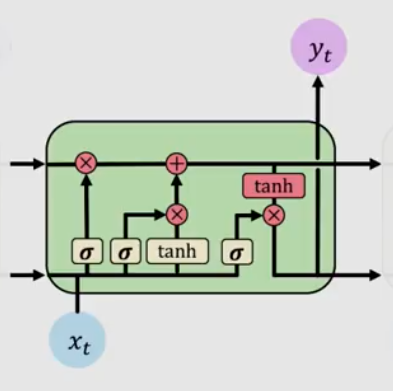
\includegraphics[width=8cm]{Images/lstm_cell.png}
\centering
\caption{LSTM Cell}
\end{figure}


\section{Convolution Neural Networks and Image Data}

\subsection{Nearest Neighbours}

Image classification is an involved method of learning from large amounts of raw data. A basic method to classify images is to memorize all the elements in the training set, and run a $L_1$ distance (Manhattan distance) comparison of the predict example through all elements of the set, and output the example with the least distance. We can also use the $L_2$ distance (Euclidean distance) to evaluate the same. Hence, this method is called a nearest neighbour classifier, as it finds the closest image to the one to be predicted and assumes they're of the same class. One problem of this approach is when the predictions start sucking up to data, this causes the classification to heavily overfit. To reduce the effect of this, we modify our algorithm to consider the k-nearest neighbours, and take a vote among them. This will smooth out the decision boundaries and give a better result. One major downfall of this algorithm, however is that the training of the algorithm is $\mathcal{O}(1)$ where the simple goal is to memorise the data. The evaluating of the algorithm, however, is $\mathcal{O}(n)$ which is not preferable, as generally, training time is flexible, and can be large, but evaluation is supposed to be fast.

To address the flaws of the k-nearest neighbours classifier, a new technique called convolutional neural networks was developed. The features from an image were identified and marked out, which resulted in significantly fewer parameters, and faster computation, even for large images.

\subsection{Feature Extraction}

It helps to think of an image as a function, $I(x, y)$, where $I$ is the image function, with two axes, $x$ and $y$. For a color image, using 3 color channels - red, green and blue, we could represent the image function as a 3 component vector. 
$$I(x, y) = \begin{bmatrix}
r(x, y)\\g(x, y)\\b(x, y)
\end{bmatrix}$$
From this, we can also think of an image as a matrix and extract features from the image to learn from with this. We can consider a moving average over the image, with a mask or a filter that slides over the image. This process is called correlation filtering. With an filter of size $2k+1 \times 2k+1$, the average can be taken across the whole image. This can be represented mathematically as follows.
$$G[i, j] = \frac{1}{(2k+1)^2} \sum_{u=-k}^k \sum_{v=-k}^k F[i+u, j+v]$$
Here we assume that the filter has all uniform weights, but this need not be the case in reality, accounting for which, the equation is modified as follows. 
$$G[i, j] = \sum_{u=-k}^k \sum_{v=-k}^k H[u, v] F[i+u, j+v]$$
Non uniform weights are also better as they may not have discrete sharp cutting edges like a uniform square filter. A Gaussian filter would be a smooth filter which accurately represents a blurry dot, a single point of light from afar, but out of focus. The smoothing filter hence would be proportional to $exp(- \frac{u^2 + v^2}{2 \sigma ^2})$.
Similarly, we can also perform an operation known as convolution. Convolution is when we flip the kernel mask before performing the correlation operation, and it would have the following change in the equation. The convolution operation DOES NOT differ from the correlation operation for a symmetric kernel. 
$$G[i, j] = \sum_{u=-k}^k \sum_{v=-k}^k H[u, v] F[i-u, j-v]$$
This operation is shift invariant - meaning it doesn't depend on the position of the filter with respect to the image, rather only on the pixels in the neighbourhood of the image. Some larger kernels enjoy a property called separability, which is of use in saving computational operations. A filter $H$ can be made by convolving a filter $c$ which is a column vector of sorts, with a filter $r$, a row vector. As the convolution property is associative, $G = H*F = (c*r)*F = c*(r*F)$ which can save up on multiplication expenses for larger kernels.

\subsection{Edge Detection}

The edges in an image convey a lot of information about it. But the edges also truncate a lot of data from the image - giving us a sort of compressed image to work with. So finding edges in an image may be very useful for speeding up computation. We can start with the idea of a normalization coefficient. Borrowing the mask or the kernel from the previous subsection, we slide it through the image and calculate the correlation between the image and the kernel. The parts where the kernel matches with the original image would get accentuated in the output. 

The original image matrix can be filtered into an edges matrix by performing a convolution operation on it with a kernel or a filter matrix. A convolution operation is performed by element wise multiplication and addition of terms resulting from it. For example, consider the image below, which is light on the left and dark on the right. Convoluting it with a vertical edge filter shows in the result, which indicates a vertical edge in the middle.
$$\begin{bmatrix}
1 & 1 & 1 & 0 & 0 & 0\\
1 & 1 & 1 & 0 & 0 & 0\\
1 & 1 & 1 & 0 & 0 & 0\\
1 & 1 & 1 & 0 & 0 & 0
\end{bmatrix}
*
\begin{bmatrix}
1 & 0 & -1\\
1 & 0 & -1\\
1 & 0 & -1
\end{bmatrix}
$$$$
=
\begin{bmatrix}
1+1+1+0+0+0-1-1-1 & 1+1+1+0+0+0+0+0+0 & ... & ...\\
1+1+1+0+0+0-1-1-1 & 1+1+1+0+0+0+0+0+0 & ... & ...\\
\end{bmatrix}
$$$$
=
\begin{bmatrix}
0 & 3 & 3 & 0\\
0 & 3 & 3 & 0\\
\end{bmatrix}$$

There are a variety of filters to use for edge detection, like the Sobel filter or the Scharr filter, below respectively.
$$
\begin{bmatrix}
1 & 0 & -1\\
2 & 0 & -2\\
1 & 0 & -1\\
\end{bmatrix}
or
\begin{bmatrix}
3 & 0 & -3\\
10 & 0 & -10\\
3 & 0 & -3\\
\end{bmatrix}
$$

\subsection{Convolutions}

For an image of size $m \times n$, convoluted with a $f \times f$ filter, the output matrix is of size $m-f+1 \times n-f+1$. This type of convolution is called valid convolution, with some loss of data near the edges of the image. To prevent this loss, same convolution can be done, where the size of the output image is same as the original. We pad the image with $p$ pixels on all of its sides, and hence have the output matrix as $m+2p-f+1 \times n+2p-f+1$. Solving this for $m \times n$ gives $p = \frac{f-1}{2}$. Note that this implies $f$ is odd, and by convention, it is so. To help with zero padding, the numpy function \code{np.pad} can be used. Another method of convoluting an image would be walk down with the filter in strides, which gives the dimensions of the output matrix as $\floor*{\frac{m+2p-f}{s} + 1} \times \floor*{\frac{n+2p-f}{s} + 1}$.

Every convolution layer accepts an input of $m \times n \times c$, and takes in four hyperparameters - the number of filters ($k$), the dimension of the filters ($f$), the stride ($s$) and the padding ($p$). This means that the output volume is of the form $\floor*{\frac{m+2p-f}{s} + 1} \times \floor*{\frac{n+2p-f}{s} + 1} \times k$. There are $f \cdot f \cdot c \cdot k + k$ learnable parameters.

\subsection{Pooling}

The pooling layer spatially downsamples the input, by reducing the height and width of the input. It helps reduce computation, as well as helps make feature detectors more invariant to its position in the input. Pooling works by sliding a filter through the input and capturing a value of the elements contained in the filter - usually maximum value or average value. Pooling also takes in a similar input to convolution, but with only two parameters - the width of the sliding frame and the stride. Generally, padding is not done for pooling. The type of pooling may also be considered, but it's generally max pooling to capture features more effectively. The output can be calculated by the same formula used for convolution. Pooling doesn't introduce any parameter, it is solely a reduction process.

\subsection{Fully Connected Layer}
After the original image is sufficiently downsampled, the result of the pooling layer is stretched out into a fully connected dense layer, and proceeds as a normal neural network seen before.


\section{Reinforcement Learning}

While standard deep learning techniques are generally supervised learning methods, reinforcement learning is a novel idea. Supervised learning follows the learn by example approach, while reinforcement learning is a learn by experience approach to a problem. To tell the RL agent whether an action it takes is good or bad, it uses a reward signal.

The reward is a scalar feedback signal at a step $t$ which talks about how well the agent is doing at that step, and the goal of the agent is to maximise cumulative reward. All goals can be described by the maximisation of expected cumulative reward. This might mean sacrificing some reward to maximise cumulative reward, as the reward can be delayed. As awards further in the future are more uncertain, they are often discounted by a discounting factor $\gamma$. The discounted cumulative expected reward is hence:
$$G_t = \sum_{n=0}^{\infty} \gamma^n R_{t+n+1}$$ where t is a time step, and $n$ tracks rewards all the way into the far future.

At every step $t$, the agent makes an action $A_t$, receives an observation $O_t$ and a reward $R_t$. The environment is the inverse, which receives the action, and emits the observation and the reward. The history $H_t$ is the sequence of actions, observations and rewards. They are all the observable variables until step $t$. 

\subsection{State}
The state, $S_t$ is information which is used to determine what happens next, and this is a function of the history. 
$$S_t = f(H_t)$$
Thus, the agent selects actions based on the history. The agent state is represented by $S_t^a$. The environment state $S_t^e$ is the environment's private representation which is usually not available to the agent. 

An information state or a Markov state contains all the useful information from the history. "The future is independent of the past given the present." A state $S_t$ is Markov if and only if:
$$P[S_{t+1}|S_t] = P[S_{t+1}|S_1, S_2, S_3, ..., S_t]$$

The state is a sufficient statistic of the future. The environment state, by definition is Markov. When the agent has full observability of the environment, $S_t^a=S_t^e$, and formally, this is a Markov decision process. But more commonly, the agent only comes across partially observable states, where the agent has to construct its own state representation. This can be the complete history, or an expectation of the environment, or a recurrent neural network. 

\subsection{RL Agent}
An RL agent may include these components.
\begin{itemize}
\item[$\square$] A policy function is the agent's behavior function. It is a map from state to action. It can be deterministic or stochastic. A deterministic policy directly maps the state to the action, like as $a = \pi(s)$. A stochastic policy outputs a probability distribution over actions instead, and works as $\pi(a|s) = P[A=a|S=s]$.
\item[$\square$] A value function, which evaluates how good or bad each state is, and can serve as a prediction of future reward. The agent will pick the state with the largest value to go to the next step.
$$v_{\pi}(s) = \mathbb{E}_{\pi}[R_t + \gamma R_{t+1} + \gamma^2 R_{t+2} + ... | S_t = s]$$
\item[$\square$] A model, which is the agent's representation of the environment. It predicts what the environment is going to do next. $\mathcal{P}$ predicts the next state, and $\mathcal{R}$ predicts the next reward.
\end{itemize}

\subsubsection{Monte Carlo vs Temporal Difference}

When an agent learns through a Monte Carlo approach, it completes one episode, or reaches one terminal state first. It now looks back and determines how its journey was and evaluates its total reward. Now it starts a new episode with the added information.
$$V(S_t) = V(S_t) + \alpha\left(G_t - V(S_t)\right)$$

Temporal difference models aren't as patient as Monte Carlo ones and update their value functions after any time-step where they reach a new state. It will update its value estimation $V$ for the non-terminal states $S_t$ occurring at that experience.
$$V(S_t) = V(S_t) + \alpha\left(R_{t+1} + \gamma V(S_{t+1} - V(S_t)\right)$$

\subsubsection{Exploration Exploitation Trade-Off}
Exploration is the process by which an algorithm explores a new environment and finds out more information about it. Exploitation is when the algorithm makes use of known information and uses it to maximise the reward. If the focus is on rewards for an agent, it will focus only on the nearest source of rewards and keep exploiting it repeatedly. In doing so, it might avoid a larger reward later, or it might just get stuck in an endless loop. This is why it is important for the agent to explore. This can be done with the $\epsilon$-greedy approach. Here, the model chooses to exploit with a probability of $\epsilon$ and chooses to explore with a probability of $1-\epsilon$.

\subsection{Q-Learning}
Q-learning is an off policy reinforcement learning algorithm that seeks to find the best action to take given the current state. It uses a Q-function (quality function) which takes two inputs: state and action. It returns the expected future reward of that action at that state.
$$Q^{\pi}(s_t, a_t) = \mathbb{E}_{\pi}[R_t + \gamma R_{t+1} + \gamma^2 R_{t+2} + ... |s_t, a_t]$$
The Q-learning algorithm works as follows. First a Q table is initialised, either with random values or with zeros. With the Q table, an action is taken given the current state and the reward is observed. The Q table is then updated as:
$$Q(s, a) = Q(s, a) + \alpha \left[R(s, a) + \gamma \max Q'(s', a') - Q(s, a) \right]$$
$Q'$ is the maximum expected future reward given the new state and all possible actions which can be taken at that state.

\subsubsection{Deep Q Learning}
Deep Q learning is when we use deep feed forward neural networks to approximate the Q values for the Q function rather than determining it accurately. This proves to be particularly useful in cases where the Q table can be very large, when the system has a lot of possible actions or a lot of possible states. However, one problem which can arise from approximating the functions is unstable learning. The same parameters are used for estimating the Q values and the target values from the Bellman equation. Hence, the target values also shift as the Q values shift. To prevent this, we can used fixed weights during training. The target network is evaluated with fixed parameters $W^-$ which are updated every $\tau$ steps.

\subsubsection{Double DQN}
At the beginning of training, since the Q table is initialised randomly or with zeros, we don't have enough information about the best action to take. This may result in the agent chasing a sub-optimal case with false positives. To prevent this, we decouple the action selection from the target value selection with two networks. A target network is used to calculate the target Q value of taking an action at a given state. A standard DQN network picks the action which the agent actually takes. This helps in reducing overestimation of Q values and hence, helps in faster and more stable training.

DDQN
PER

\subsection{Policy Based Learning}












\end{document}
